\section{数据下载}
\subsection{安装下载工具}
\begin{frame}
    \frametitle{打开浏览器}
    浏览器输入IDM官网网址
    \url{https://www.internetdownloadmanager.com/}\\
    按键盘上的Enter键或用鼠标点击访问。切忌从xx下载站下载
    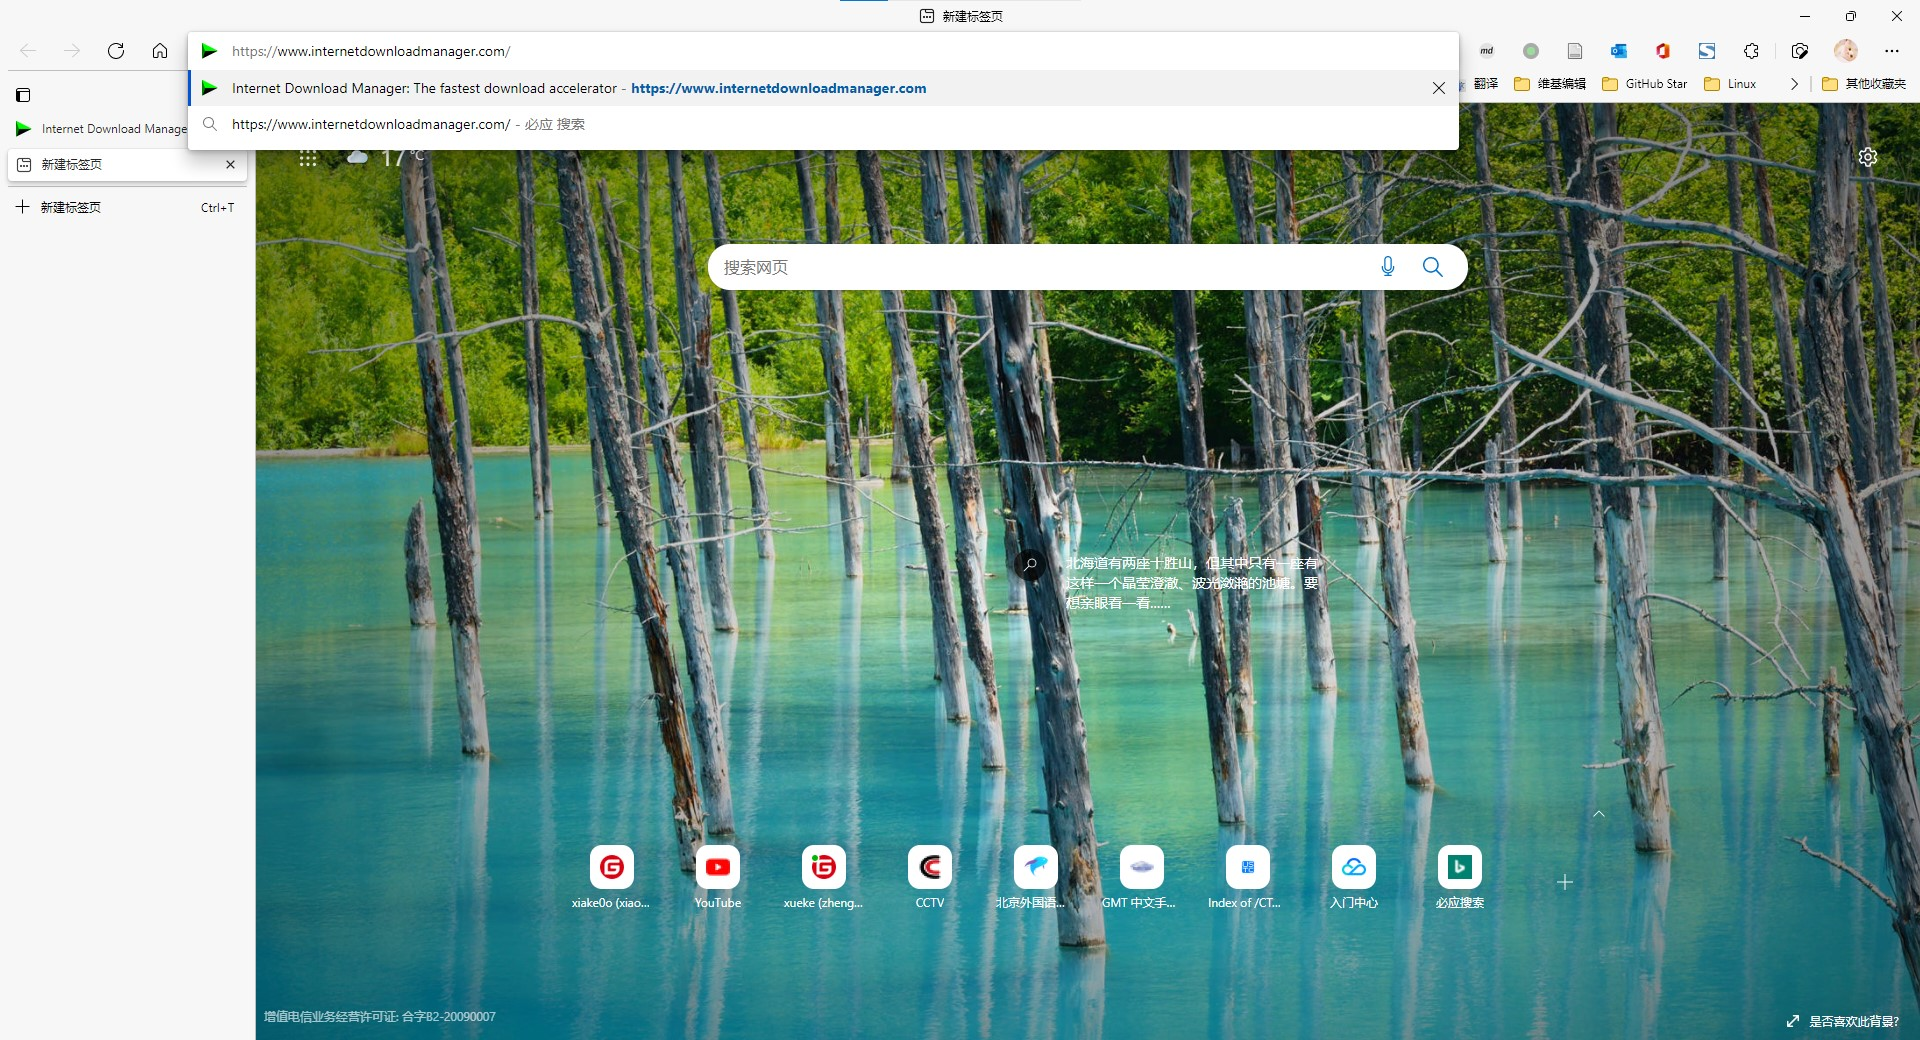
\includegraphics[width=\linewidth]{images/21.IDM网址.jpg}
\end{frame}
\begin{frame}
    \frametitle{下载IDM}
    点击 \underline{TRY IDM 30-DAYS FREE TRIAL}下载
    \begin{annotationimage}{width=\linewidth}{images/22.IDM官网}
        \draw[red,very thick](0.42,0.54) rectangle (0.58,0.6);
    \end{annotationimage}
\end{frame}
\begin{frame}
    \frametitle{安装IDM}
    打开下载好的安装包,一路Next就好。
    安装完打开长这样。
    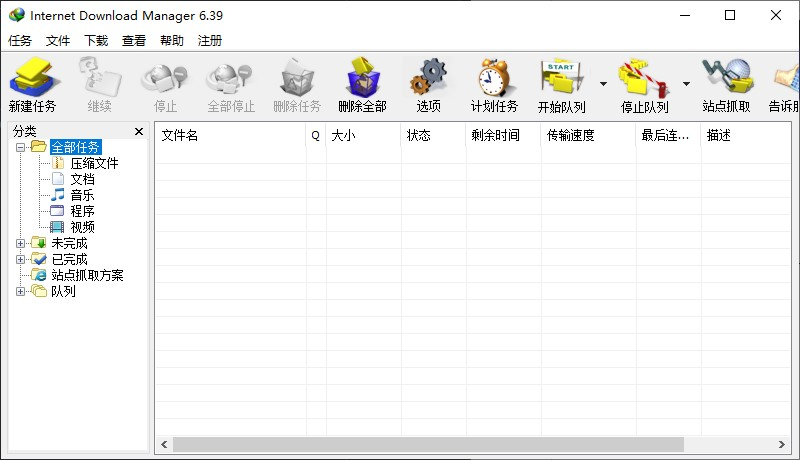
\includegraphics[width=\linewidth]{images/23.IDM长这样}
\end{frame}
\begin{frame}
    \frametitle{进入IDM设置界面}
    点击 \underline{选项按钮}
    \begin{annotationimage}{width=\linewidth}{images/23.IDM长这样}
        \draw[red,very thick](0.50,0.74) rectangle (0.58,0.89);
    \end{annotationimage}
\end{frame}
\begin{frame}
    \frametitle{添加文件类型}
    \begin{columns}
        \begin{column}{.5\linewidth}
            点击 \underline{文件类型}\\追加NC和HDF,用空格隔开
        \end{column}

        \begin{column}{.5\linewidth}
            \begin{annotationimage}{width=\linewidth}{images/42.添加文件类型}
                \draw[red,very thick](0.16,0.88) rectangle (0.35,0.92);
                \draw[red,very thick](0.18,0.67) rectangle (0.28,0.70);
            \end{annotationimage}
        \end{column}
    \end{columns}
\end{frame}
\subsection{获取链接}
\begin{frame}
    \frametitle{全选订单文件}
    回到我们的订单内容页面
    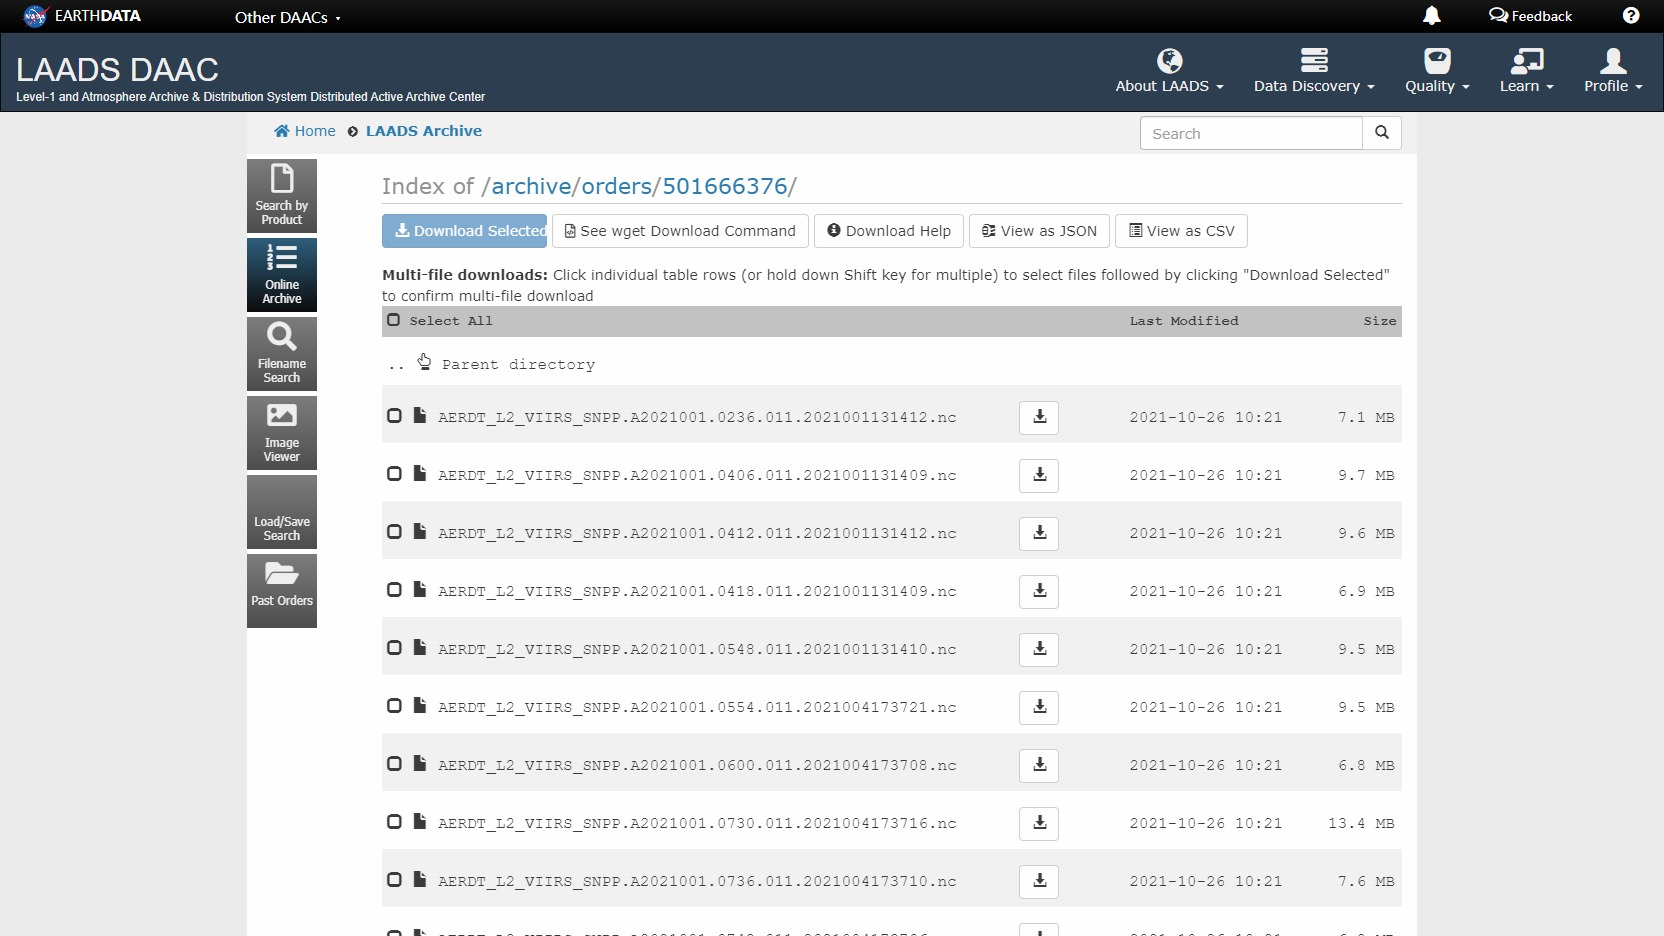
\includegraphics[width=\linewidth]{images/20.订单内容}
\end{frame}
\begin{frame}
    \frametitle{选中全部订单文件}
    点击\underline{Select All}复选框,选中全部文件
    \begin{annotationimage}{width=\linewidth}{images/20.订单内容}
        \draw[red,very thick](0.23,0.64) rectangle (0.3,0.68);
    \end{annotationimage}
\end{frame}
\begin{frame}
    \frametitle{获取选中文件地址}
    点击\underline{Download All}按钮,获取选中文件的存储链地址
    \begin{annotationimage}{width=\linewidth}{images/24.全选订单文件}
        \draw[red,very thick](0.23,0.73) rectangle (0.33,0.77);
    \end{annotationimage}
\end{frame}
\begin{frame}
    \frametitle{全选文件地址}
    使用鼠标选中所有文件地址并复制\\
    但这不是可以直接下载的地址,所以请继续下一步
    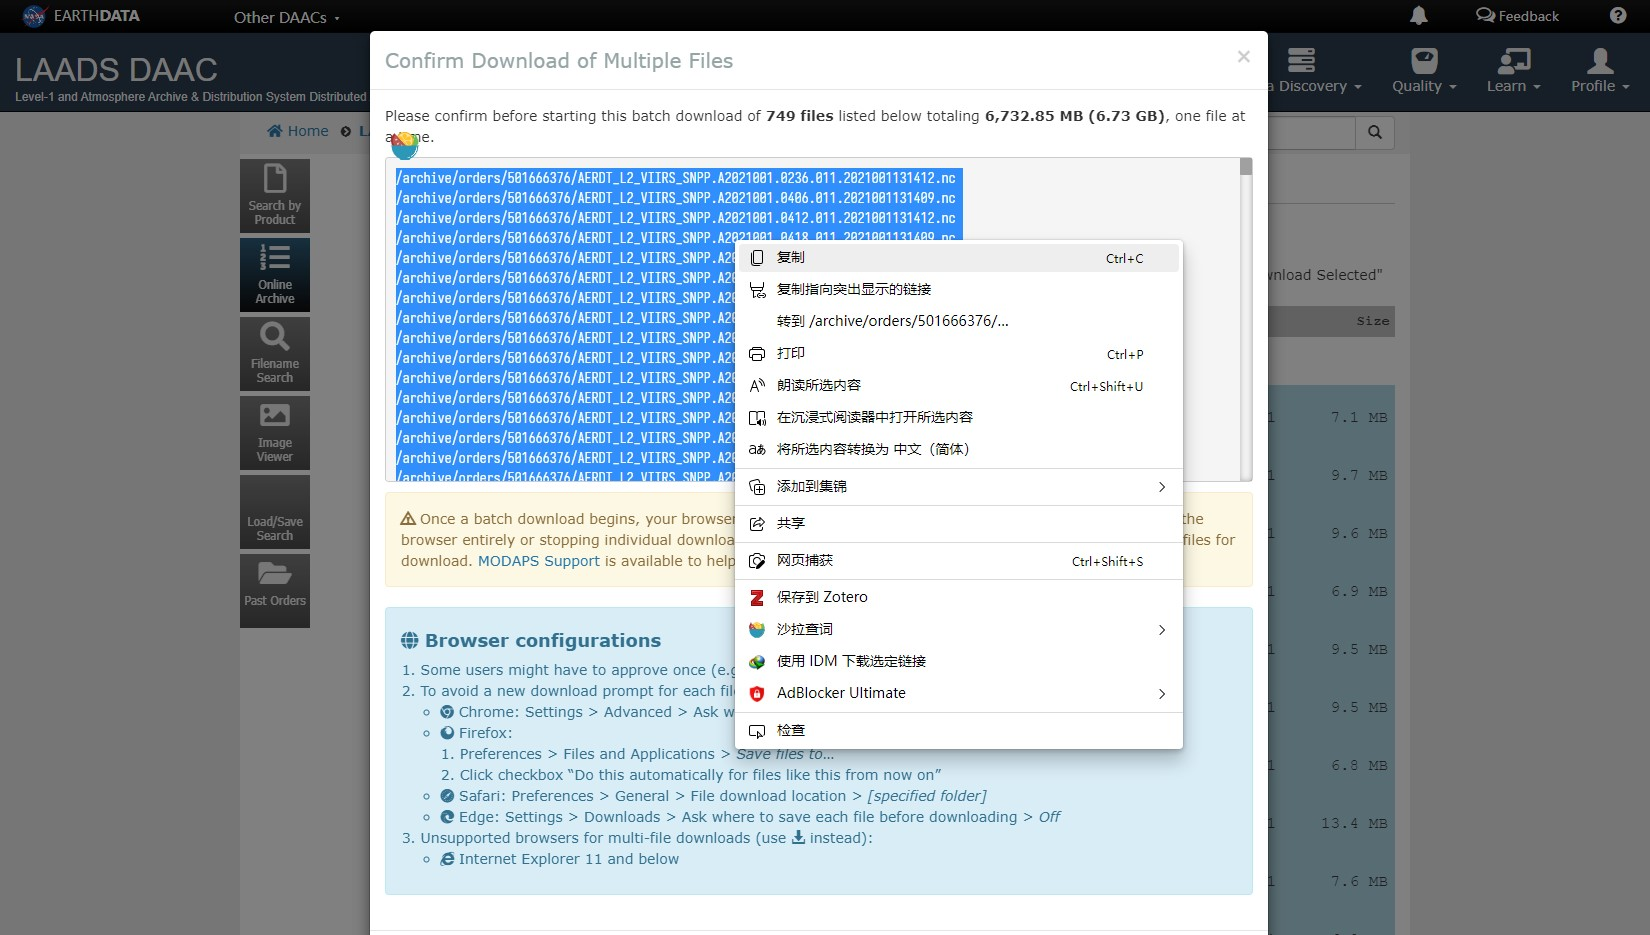
\includegraphics[width=\linewidth]{images/25.全选文件地址}
\end{frame}
\begin{frame}
    \frametitle{建立一个文件夹}
    找个清楚的地方新建一个文件夹,用来存放待下载的文件\\
    假如叫laads\_order\_501666376
    \begin{annotationimage}{width=\linewidth}{images/26.新建一个文件夹}
        \imagelabelset{image label back = white,image label text = black}
        \draw[image label = {推荐阁下也以这样的方式命名,其中501666376是该订单的订单号 at center}];
    \end{annotationimage}
\end{frame}
\begin{frame}
    \frametitle{存储文件地址}
    在该文件夹下新建一个文本文件,假如叫file\_download\_link.txt,将刚才复制的文件地址粘贴进来
    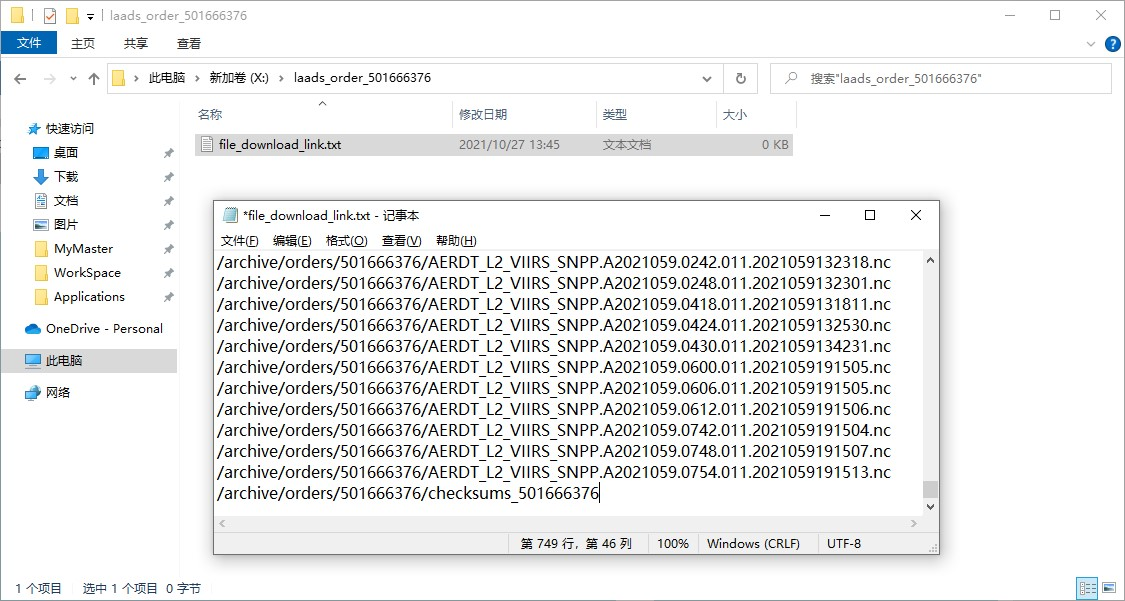
\includegraphics[width=\linewidth]{images/27.粘贴下载链接}
\end{frame}
\begin{frame}
    \frametitle{使用替换工具完善文件地址}
    在每个文件地址的开头加上https://ladsweb.modaps.eosdis.nasa.gov即为其真正的下载
    地址,我们使用替换工具实现这一目的
    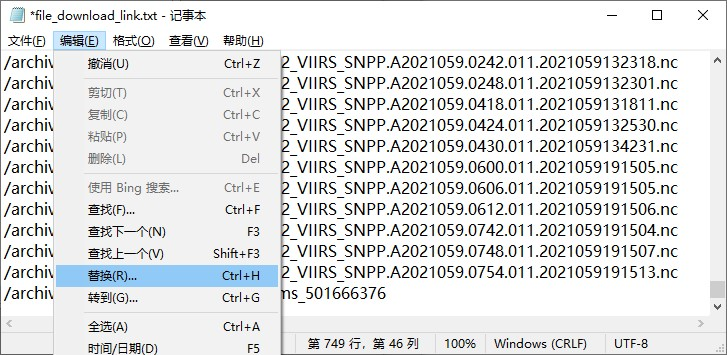
\includegraphics[width=\linewidth]{images/28.替换工具}
\end{frame}
\begin{frame}
    \frametitle{执行替换操作}
    查找内容:/archive\\
    替换为:https://ladsweb.modaps.eosdis.nasa.gov/archive \\
    执行\underline{全部替换},即可达到目的
    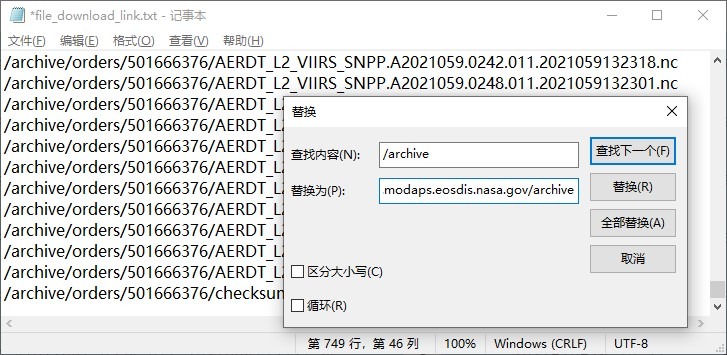
\includegraphics[width=\linewidth]{images/29.替换项目}
\end{frame}
\begin{frame}
    \frametitle{替换结果}
    这样我们就得到了订单中所有文件的真实下载地址
    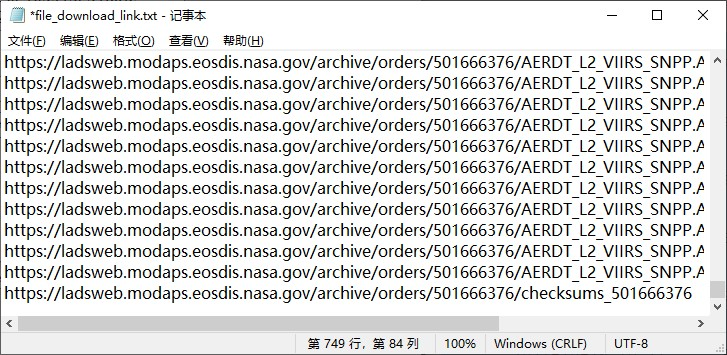
\includegraphics[width=\linewidth]{images/30.替换结果}
\end{frame}
\begin{frame}
    \frametitle{保存文件下载地址}
    将文件保存以备后续下载使用
    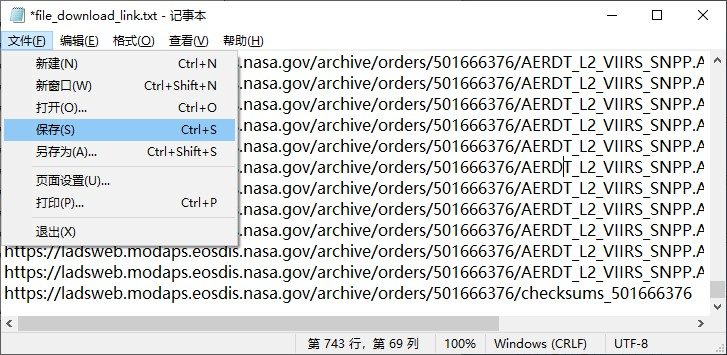
\includegraphics[width=\linewidth]{images/31.保存替换结果}
\end{frame}
\subsection{新建任务队列}
\begin{frame}
    \frametitle{创建下载队列}
    在IDM界面右键队列,选择创建队列。\\
    创建队列的目的在于可以对下载任务进行集中管理。
    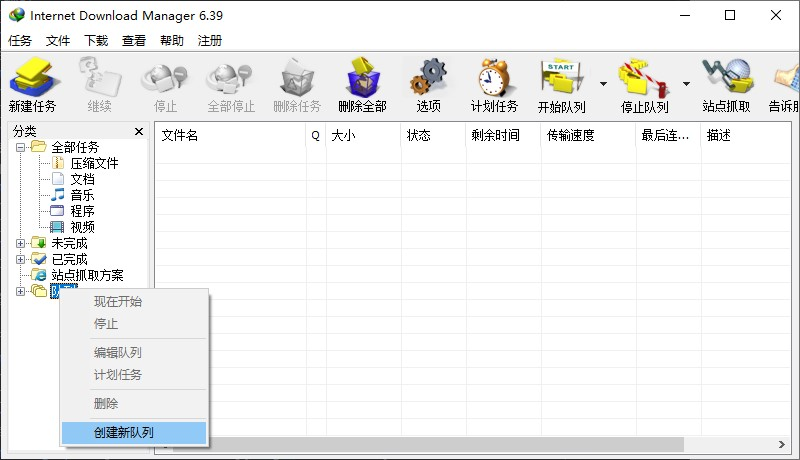
\includegraphics[width=\linewidth]{images/32.创建队列}
\end{frame}
\begin{frame}
    \frametitle{设置队列名}
    给该队列起一个有意义的名字(随意,这样只是为了好辩认)
    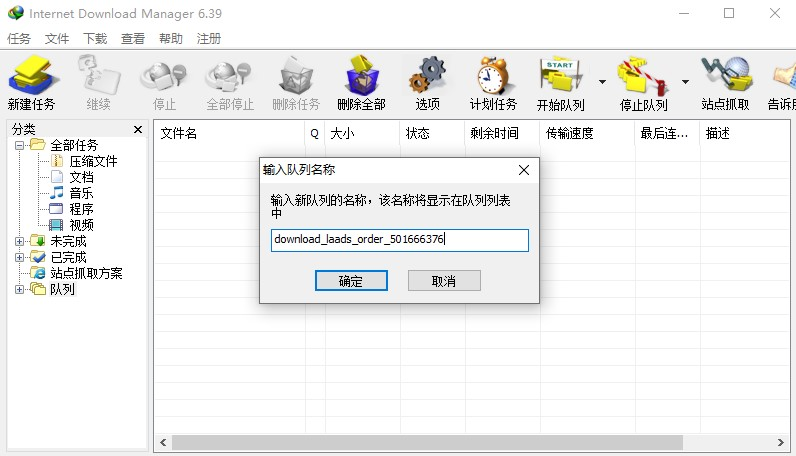
\includegraphics[width=\linewidth]{images/33.设置队列名}
\end{frame}
\begin{frame}
    \frametitle{设置队列重试次数}
    勾选失败后重试次数,保持默认值10即可
    \begin{figure}
        \begin{annotationimage}{width=0.65\linewidth}{images/43.设置重试次数}
            \draw[red,very thick] (0.3,0.36) rectangle (0.91,0.43);
        \end{annotationimage}
    \end{figure}
\end{frame}
\begin{frame}
    \frametitle{设置下载队列属性}
    默认队列同一时间只能下载一个文件\\
    我们这里设置为可以同时下载5个。分别点击 \underline{应用}和 \underline{关闭}
    \begin{figure}
        \centering
        \begin{annotationimage}{width=0.65\linewidth}{images/34.设置队列属性}
            \draw[red,very thick] (0.34,0.80) rectangle (0.58,0.88);
            \draw[red,very thick] (0.66,0.01) rectangle (0.77,0.07);
            \draw[red,very thick] (0.78,0.01) rectangle (0.89,0.07);
            \draw[coordinate label = {1 at (0.46,0.91)}];
            \draw[coordinate label = {2 at (0.715,0.1)}];
            \draw[coordinate label = {3 at (0.835,0.1)}];
        \end{annotationimage}
    \end{figure}
\end{frame}
\subsection{导入下载链接}
\begin{frame}
    \frametitle{刷新订单页面}
    在开始下载之前,需要刷新一下订单详情页,这样可以让IDM捕获到缓存的LAADS用户授权信息
    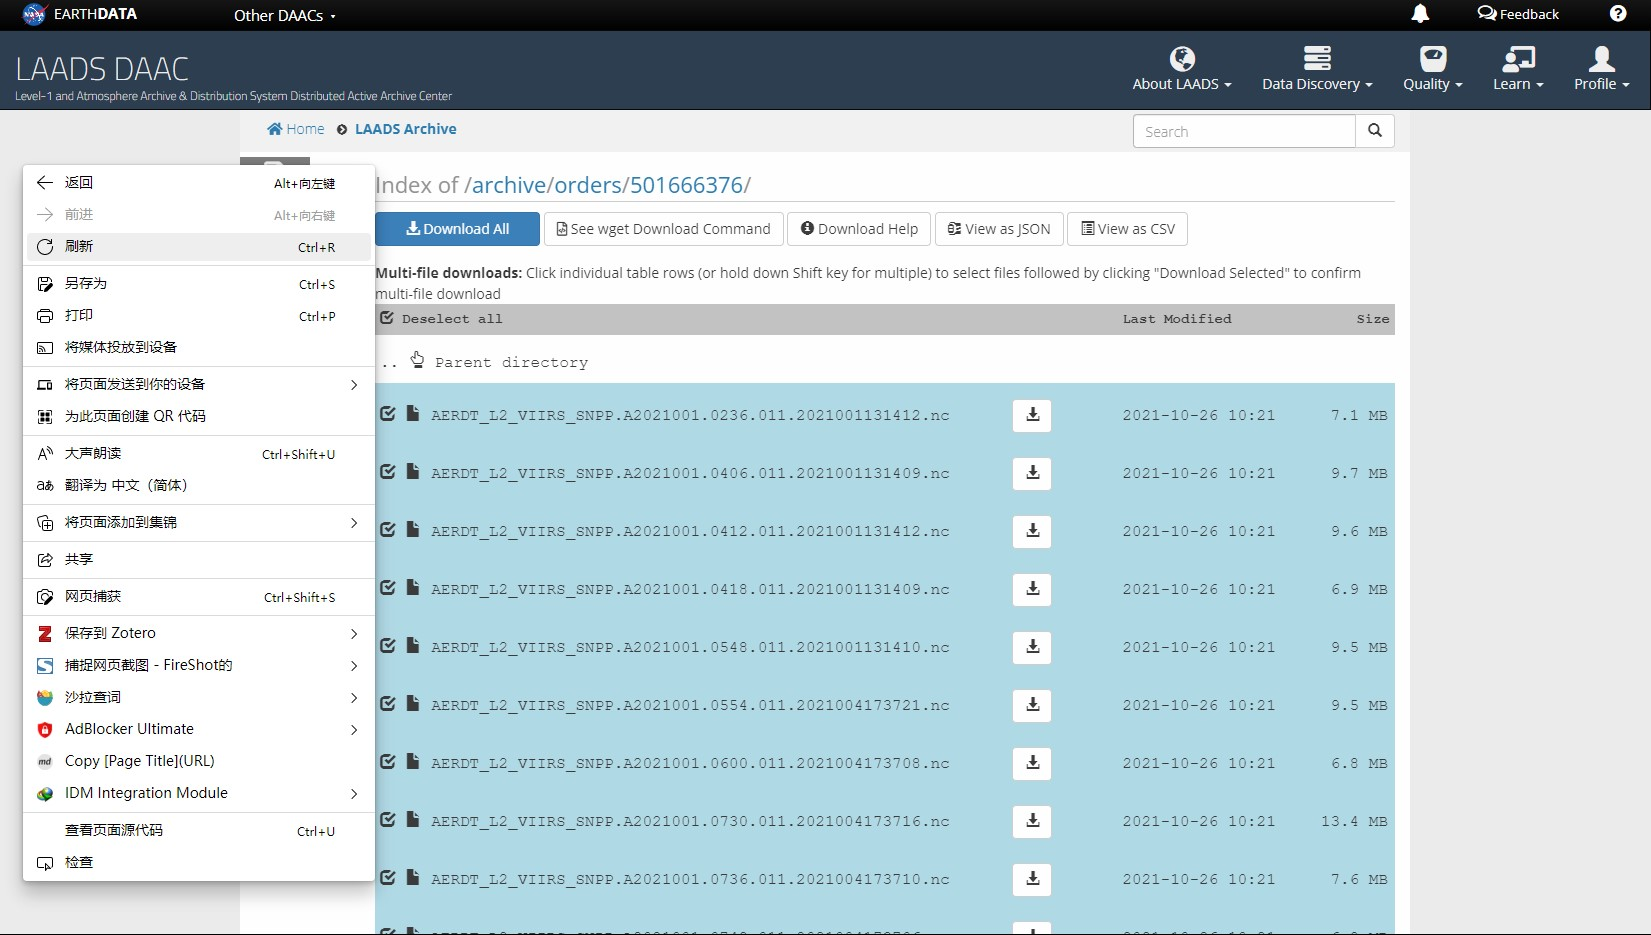
\includegraphics[width=\linewidth]{images/37.刷新一下订单页面.jpg}
\end{frame}
\begin{frame}
    \frametitle{导入下载地址}
    选择从文本文件导入,导入我们刚才创建的文件下载地址文件
    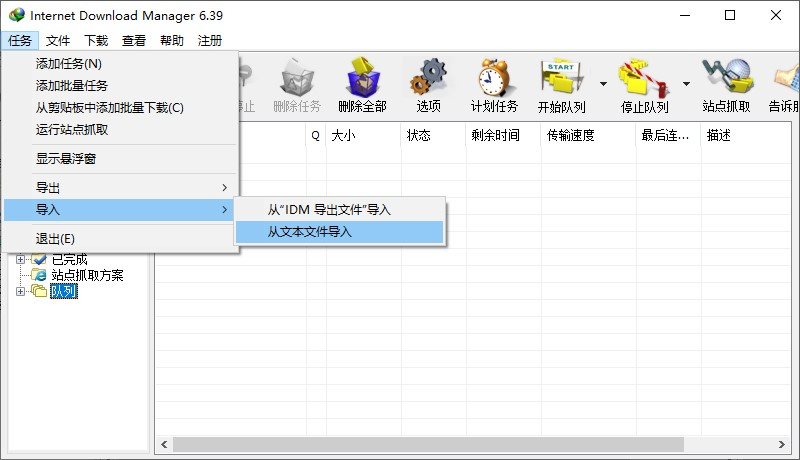
\includegraphics[width=\linewidth]{images/35.导入下载链地址}
\end{frame}
\begin{frame}
    \frametitle{选择我们创建的下载地址文件}
    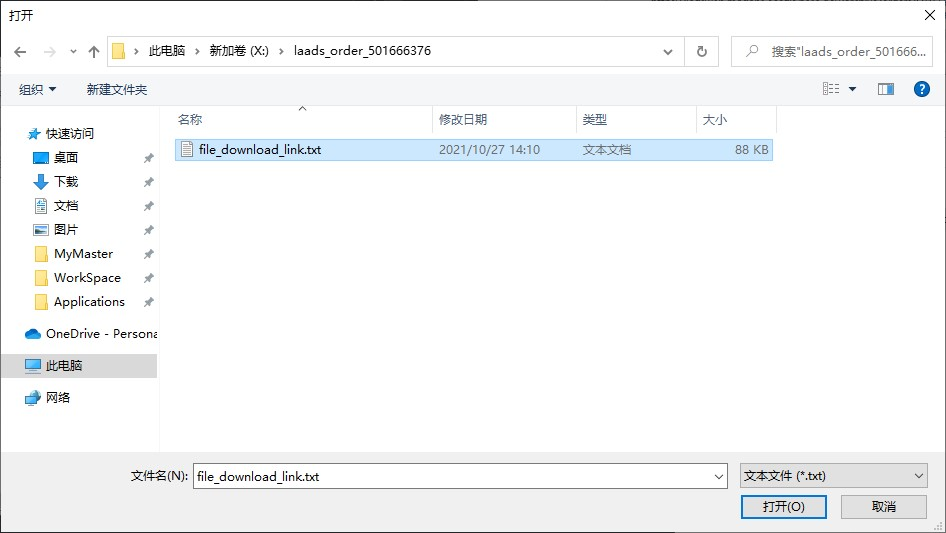
\includegraphics[width=\linewidth]{images/36.选择下载链接文件}
\end{frame}
\begin{frame}
    \frametitle{导入效果}
    如果正确识别出了文件类型和大小,则表示没有问题
    \begin{enumerate}
        \item 点击浏览,选择我们新建的存储文件夹
        \item 点击全部选择,勾选全部文件
        \item 点击确定
    \end{enumerate}
    \begin{figure}
        \begin{annotationimage}{width=0.65\linewidth}{images/38.导入结果}
            \draw[red,very thick] (0.17,0.28) rectangle (0.44,0.88);
            \draw[red,very thick] (0.02,0.03) rectangle (0.52,0.12);
            \draw[red,very thick] (0.58,0.20) rectangle (0.70,0.25);
            \draw[red,very thick] (0.77,0.01) rectangle (0.87,0.07);
            \draw[coordinate label = {1 at (0.27,0.15)}];
            \draw[coordinate label = {2 at (0.64,0.28)}];
            \draw[coordinate label = {3 at (0.82,0.10)}];
        \end{annotationimage}
    \end{figure}
\end{frame}
\subsection{下载}
\begin{frame}
    \frametitle{添加到队列}
    \begin{enumerate}
        \item 弹出队列选择,选择我们新建的队列
        \item 勾选\underline{开始执行队列}
        \item 点击确定,开始下载
    \end{enumerate}
    \begin{figure}
        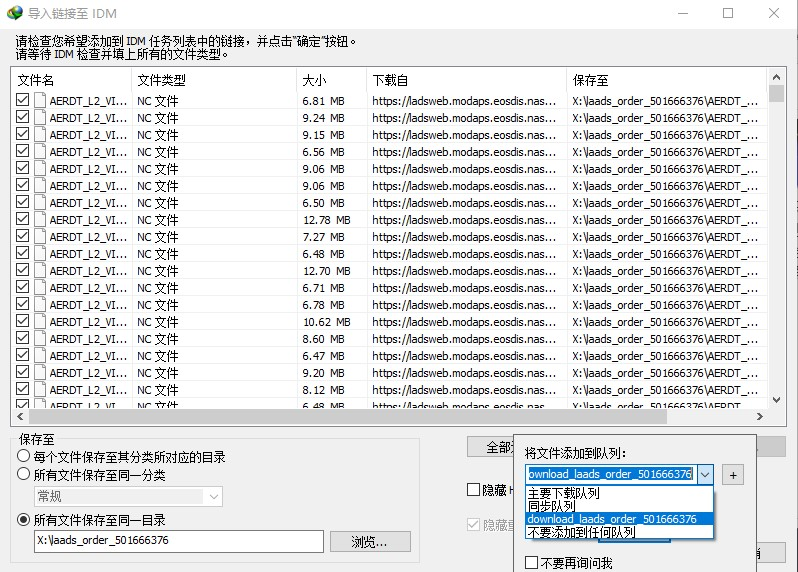
\includegraphics[width=0.65\linewidth]{images/39.添加到队列}
    \end{figure}
\end{frame}
\begin{frame}
    \frametitle{下载中...}
    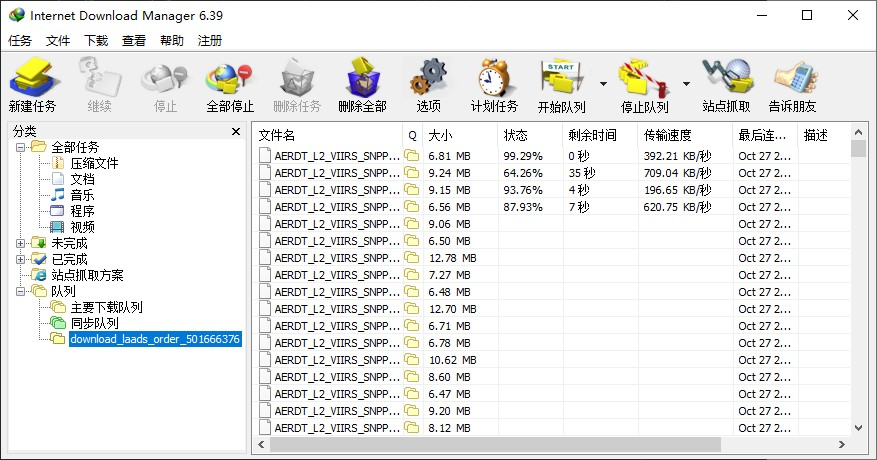
\includegraphics[width=\linewidth]{images/40.下载中}
\end{frame}
\begin{frame}
    \frametitle{有错误怎么办?}
    不要紧,我们已经设置过重试次数了\\
    \begin{itemize}
        \item 如果阁下想手动刷新,可以右键错误项,选择 \underline{继续下载}
        \item 点击 \underline{状态},可以将正在下载的文件提到列表前面\\
        \item 如果没有一个文件处于下载状态,建议阁下刷新一下浏览器中的订单详情界面,
              以免登陆状态失效
    \end{itemize}
    \begin{figure}
        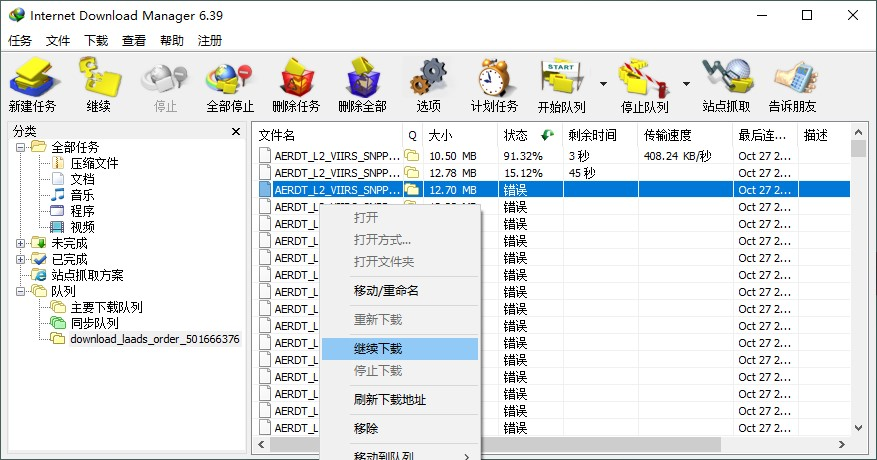
\includegraphics[width=.8\linewidth]{images/41.有错误.jpg}
    \end{figure}

\end{frame}